\chapter{Results and Analysis}
This chapter provides a graphical representation of the data acquired from conducting the tests designed in the last chapter. The raw data used to generate this graphs can be accessed in \hyperref[AppendixB]{Appendix B}. After the graphs their analysis is done to explain the various characteristics of the two wireless protocols according to the experimental results.

\section{\acrlong{ht} Test}
\subsection{Graphical Representation of the Data Acquired}
The data acquired from the different test cases of the \gls{ht} test suite is represented graphically below. Figure \ref{fig:HT-dr}, \ref{fig:HT-r} and \ref{fig:HT-ec} provides information about the measurement of data rate, reliability and energy consumption respectively. The legend used for naming the test cases is same as described in section \ref{6HTdesign}.

\begin{figure}[h]
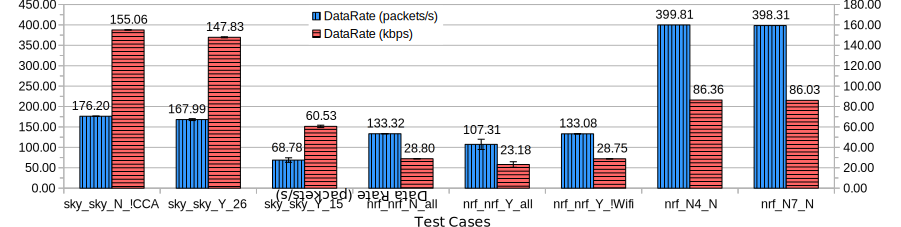
\includegraphics[width=\textwidth]{HT-dr}
\caption{Data Rate}
\label{fig:HT-dr}
\vspace{-6 pt}
\end{figure}

Note that in figure \ref{fig:HT-dr} there are two Y-axis representing the data rate in packets per second and kilobit per second. The link layer payload of 27 bytes and 110 byte was used for BLE and 802.15.4 respectively to calculate the data rate in kbps.

\begin{figure}[h]
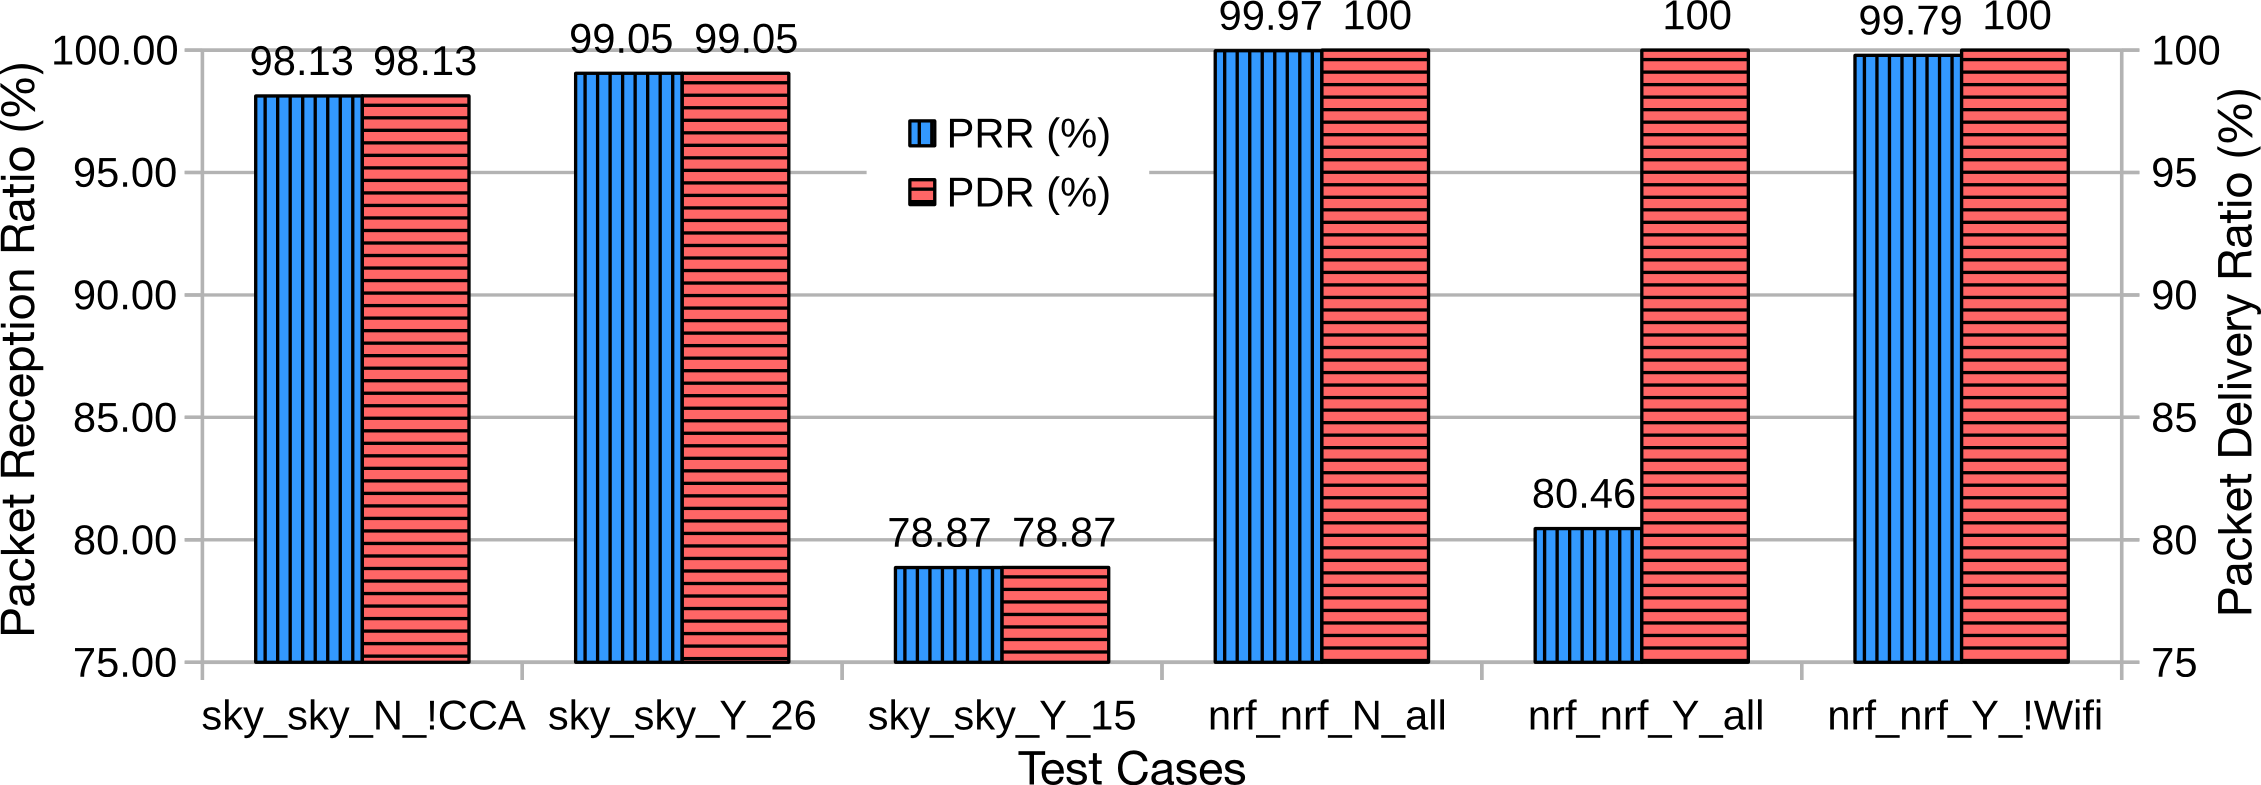
\includegraphics[width=\textwidth]{HT-r}
\caption{Reliability}
\label{fig:HT-r}
\vspace{-6 pt}
\end{figure}
The graph in figure \ref{fig:HT-r} has Y-axes from 75 to 100 \% for clearer representation of the \gls{pdr} and \gls{prr} \todo{Is this misleading?}. As mentioned in section \ref{6HTdesign} the reliability was calculate in BLE by logging the number of times the radio was switched on as this information was accessible from the SoftDevice. This allowed the calculation of \gls{prr} with one packet per connection event. Since the android devices can communicate multiple packets per connection event, the \gls{prr} could not be calculated. Hence, those test cases are not plotted.

\begin{figure}[h]
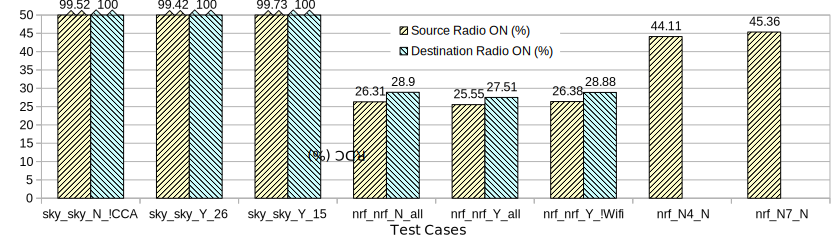
\includegraphics[width=\textwidth]{HT-ec}
\caption{Energy Consumption}
\label{fig:HT-ec}
\end{figure}

For a clearer representation of the graph, the y-axis in figure \ref{fig:HT-ec} is limited to 50\%. The break in the graph shows when Tmote-Sky uses \textasciitilde100\% of radio duty cycle. In all the tests with BLE the source node was the slave device sending the notifications, while the destination node was the master device receiving them.

There was no easy way of accessing the low level information of BLE \gls{rdc} on an Android device, so the energy consumption of these devices is not plotted. Moreover the energy consumption of such multi-purpose master device is less important than a single purpose slave device running on a meager battery.

\subsection{Analysis}
\paragraph{Data Rate}
The absolute data rate is higher in 802.15.4 than BLE although the number of packets transmitter per second is higher in BLE as seen in figure \ref{fig:HT-dr}. This is because of the higher packet size of 802.15.4 and the bit rate of transmission of BLE is four time the bit rate of 802.15.4 at 1 Mbps.

For 802.15.4 the peak data rate of 155.87 kbps is achieved when \gls{cca} is not used. The more practical approach of using \gls{cca} decreased in the data rate slightly to 148.35 kbps. When WiFi interference was introduced, most of the transmission slots were not utilized because of backing off by \gls{cca}. \hyperref[AppendixB]{Appendix B} shows that only 21\% of the transmission slots were used dropping the data rate considerably. With this 43.33  kbps data rate was achieved, which is higher than the data rate achieved by BLE communication between nodes of PCA10000 platform in any test case. Since 802.15.4's Null-RDC tries to send a packet as soon as possible, we can approximately calculate that the inference of WiFi traffic was not present 29.2\% of the time by taking the ratio of the data rate with and without WiFi interference (43.33/148.35).

The SoftDevice used to implement the central stack allows only one packet to be communicated per connection interval. With this the theoretical data rate that can be achieved can be found out by 

$\mbox{Data Rate  (packet/second)}=\frac{1}{\mbox{connection interval}}=\frac{1}{7.5ms}=133.33\:packet/second$

\vspace{15 pt}
$\mbox{Data Rate (kbps)}=\frac{\mbox{(bits per byte)}\times\mbox{(link layer payload in bytes)}}{\mbox{connection interval}}=\frac{8\times27}{7.5ms}=28.8\:kbps$
\vspace{10 pt}

The experimental results seen in figure \ref{fig:HT-dr} shows this is achieved accurately. When WiFi is introduced, the data rate drops from 28.7 kbps to 23.6 kbps, when all the channels are used. This is 82\% of the WiFi free data rate. Figure \ref{fig:Intf} shows that 10 out of the 37 data channels are interfered by WiFi traffic. This means that the data rate should reduce by (37-10)/37, which is about 73\% of the WiFi free data rate. The greater data rate achieved experimentally can be accounted to the fact that the WiFi traffic wasn't interfering 100\% of the time as inferred earlier. Considering that the 10 channels were interfered 29.2\% of the time as calculated, the data rate achievable can be calculated as $(0.292\times10/37 + 1\times27/37)\times28.8=24.1$ kbps which is closer to the achieved 23.6 kbps.

When the WiFi free channels were used the data rate recorded was close to the theoretical data rate predicted. There was no influence of the WiFi traffic at all for BLE communication in this case. This shows that when frequency hopping channel map is chosen to avoid the interference, there is no effect on the data rate.

Communication of the PCA10000 with a Nexus4/7 master device achieved a greater data rate of about 86 kbps or \textasciitilde400 packet/second. This is because the BLE stack in these Android devices support communication of multiple packets in a connection event, increasing the data rate achievable. With a connection interval of 7.5 ms, at an average there were around $(400\times7.5/1000)$ i.e. 3 packets of data received by the Android device per connection event.

\paragraph{Reliability}
In case of 802.15.4, the \gls{pdr} and \gls{prr} is same since it does not have any communication failure detection and retransmission mechanism. This is left to the upper layer to handle. The link layer just tries initiate communication when there is no external interference present with its \gls{cca}. Figure \ref{fig:HT-r} shows that the \gls{prr} achieved when \gls{cca} is switched off is 96.23\%. While it can be seen that without \gls{cca} the data-rate is higher, the reliability decreases. By using \gls{cca} in a WiFi free channel, the \gls{prr} increases to 99.55\%, which means that the \gls{cca} is effective in case of less interference. When there was heavy WiFi traffic in the same channel of communication, the \gls{cca} did work since only 21.11\% of the transmission slots were used. Of these transmissions the \gls{prr} was 84.7\%. This could happen when the interference starts after the carrier assessment, causing the packet to get corrupted. Here it can be seen that \gls{cca} of 802.15.4 has reduced effectiveness in case of heavy interference.

In case of \gls{ble}, figure \ref{fig:HT-r} shows that the \gls{pdr} is always 100\% since BLE employs a simple acknowledgment scheme to detect if the communication has not been successful so that the packet can be retransmitted. This ensures that the upper layers can safely assume that the link layer is completely reliable. Without WiFi interference \gls{prr} was about 99.64\%, which means that there were few retransmissions. With all the channels employed and with WiFi interference, the \gls{prr} reduced to 81.94\%. This number is not low because of the frequency hopping used by BLE, which ensures that interference in one frequency range only effects the communication happening over the channels in that frequency range. The other data channels can still keep the communication flow intact. This shows that the frequency hopping when used over the complete channel map helps in sustaining the communication when there is external interference. When only the WiFi free channels were employed, there was no influence of the WiFi interference on \gls{prr}, which was 99.95\%. This shows that when a master device has the capability of detecting external interference, it can adapt the frequency hopping channels so that there is negligible effect on the communication. Note that \gls{afh} can only help negate narrow band interference in the 2.4 GHz \gls{ism} band.

\paragraph{Energy Consumption}
As seen in figure \ref{fig:HT-ec}, the radio of Tmote-Sky nodes is used nearly 100\% the time in all the test cases of the \gls{ht} test suite. This shows that in 802.15.4 the data rate can be maximized, by choosing an appropriate \gls{rdc} layer like Null-RDC, although at the expense of energy consumption. 

When the test cases where the communication happened between PCA10000 node, the source node had \gls{rdc} of 25\% to 27\%. In the case \texttt{nrf\_nrf\_Y\_all} where the communication was affected by interference, the destination node had a 
\todo{redo tests for }

In case of communication with the Android devices, the source nodes had \gls{rdc} of 44\% to 45\%. This is higher because multiple packets were communicated per connection interval. With stacks supporting greater packets per connection interval, this number will increase, also increasing the throughput. This shows that when a master device can support communication of greater number packets per connection event, the data rate increases.

\section{\acrlong{rr} Test}

\subsection{Graphical Representation of Data Acquired}
\begin{figure}[h]
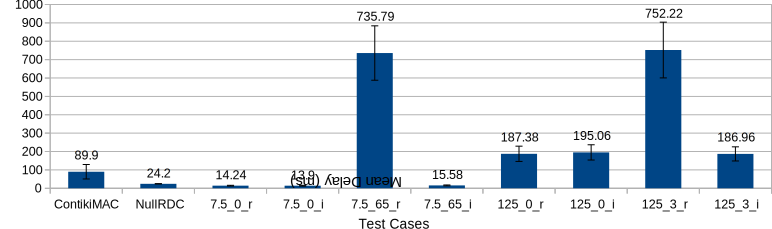
\includegraphics[width=\textwidth]{RR-l}
\caption{Latency}
\label{fig:RR-l}
\end{figure}

Figure \ref{fig:RR-l} shows the mean of the thousand measurement of latency in ms for different cases of the \gls{rr} test suite along with the standard deviation. 

\begin{figure}[h]
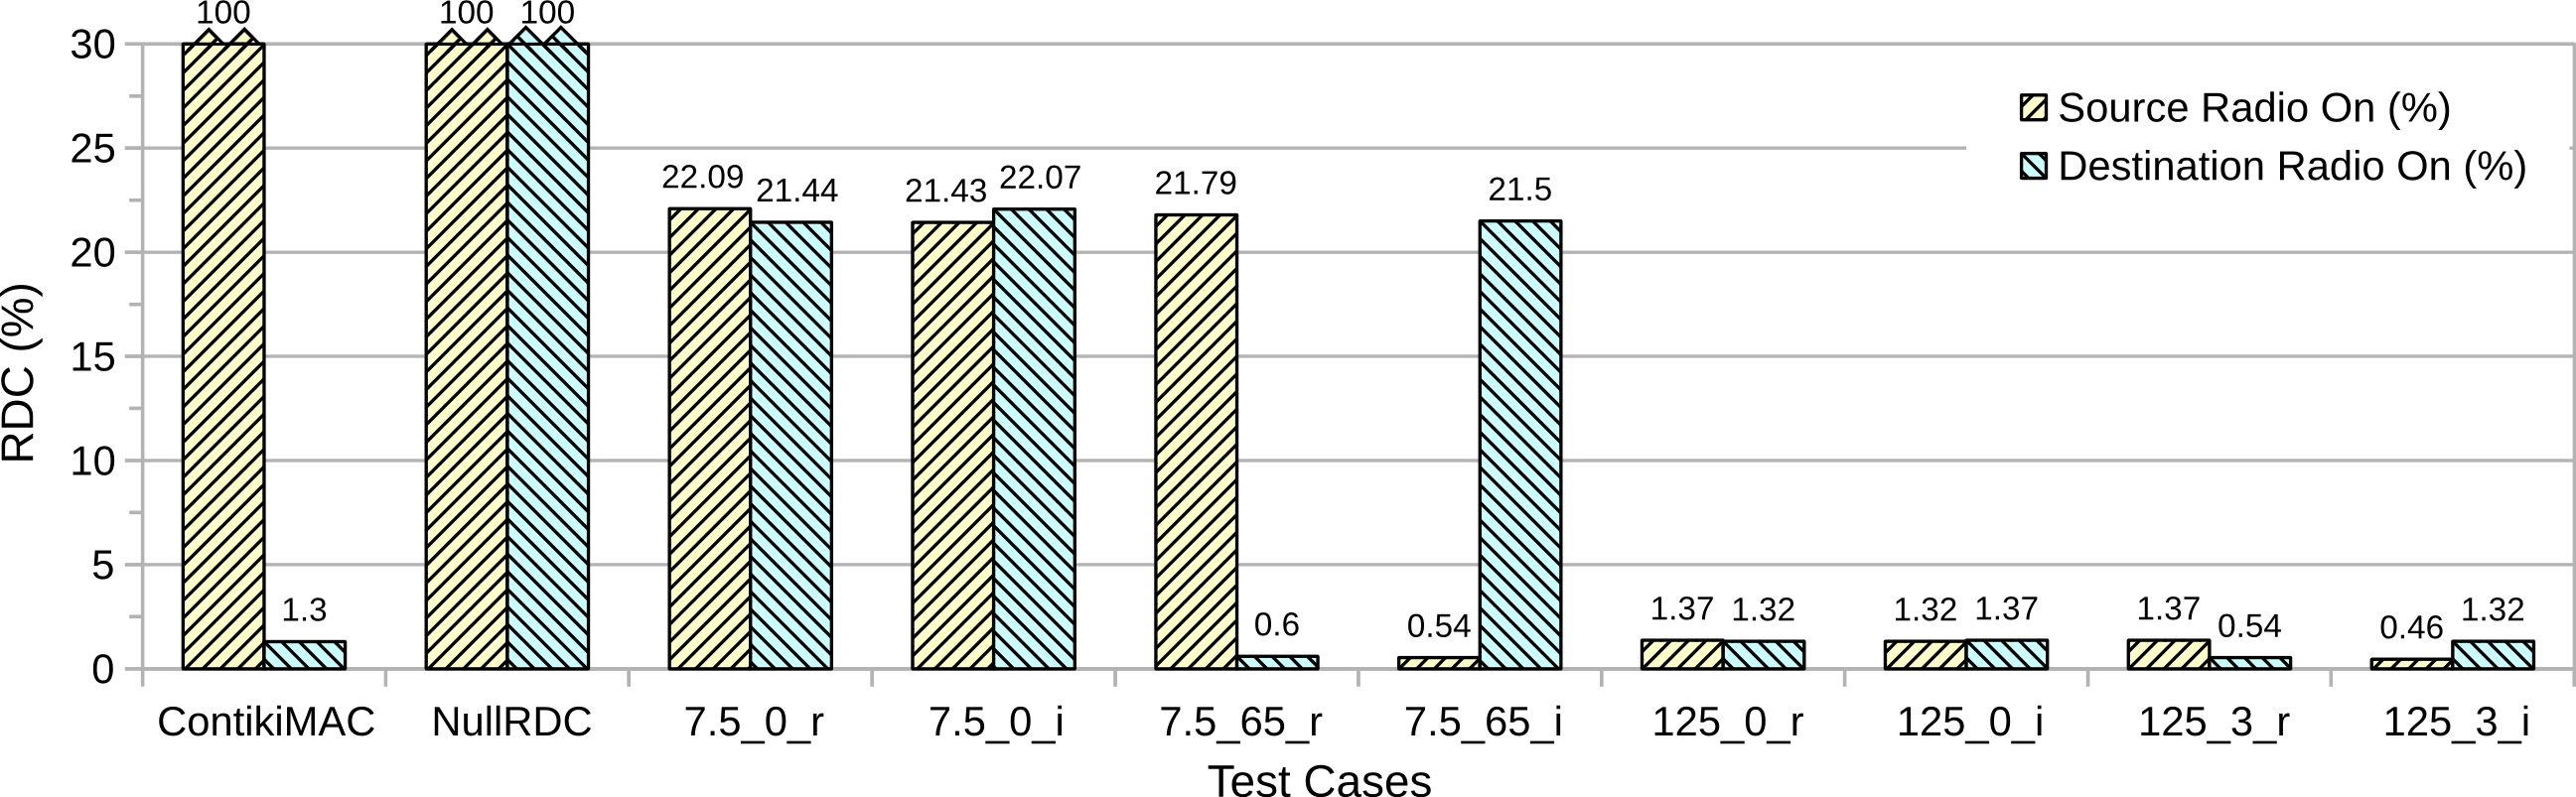
\includegraphics[width=\textwidth]{RR-ec}
\caption{Energy Consumption}
\label{fig:RR-ec}
\end{figure}

Figure \ref{fig:RR-ec} shows the energy consumption of the nodes in terms of the percentage of time the radio was switched on for the different cases of the \gls{rr} test suite. Similar to the graph for the \gls{ht} tests, this graph is limited to 30\% for clearer representation, especially of in test cases with low duty cycle.

In 802.15.4 the source and destination nodes can be identified based on who's sending and who's receiving. In case of BLE it is a bit more complicated since source and destination nodes change based on where the latency is being measured. In the tests with the master reading a packet from the slave, the master is the source while the slave is the destination. In tests with the slave sending an indication packet to the master and receiving an acknowledgment from it, the source and destination are inverted.

\subsection{Analysis}
\paragraph{Latency}
The latency measurement as seen from figure \ref{fig:RR-l} can vary in the order of magnitude among different tests. The least latency can be achieved using 802.15.4 when using Null-RDC, which is about 24 ms.  When using ContikiMAC, the average latency was about 90 ms, which can be attributed to the 125 ms interval with which the receiver wakes up. \todo{resposne in the same ack is happening, always possible?}.  \todo{update link layer config while running or is it hard coded?}

Based on the link layer configurations used for BLE, the latency varied from a minimum of about 14 ms to a maximum of about 750 ms. The provision in BLE's link layer for changing these configurations while in a connection is an advantage since the latency can be adapted according to the requirement. The configuration of the slave latency value determines if there is any difference in the latency experienced based on whether the communication happens with a read request or an indication. With slave latency as zero, the latency of the read and indication case is almost same, with the average latency being around 14 ms with 7.5 ms connection interval and 190 ms with a connection interval of 125 ms. With a non-zero slave latency value, the read-request from the master node (client in \gls{att}) has high latency since the slave node (server at \gls{att})will not react to the master at every connection interval as it is sleeping. With a slave latency value of 65, the master node can read a value from the slave node with a latency of about 736 ms, even with a connection interval of 7.5 ms. Similarly, with a slave latency of 3 and connection interval of 125 ms, the master will read a value from the slave with a latency of about 752 ms. When using indication to communicate data to a master, the latency can be low since the slave can decide to respond to the master when necessary communicate. With a 7.5 ms connection interval and slave latency of 65, the latency is about 15 ms, which is similar to the latency experience with zero slave latency. Similarly, an indication providing the master with data experiences a latency of 187 ms with a connection interval of 125 ms and slave latency of 3. This is almost equal to the latency experienced with zero slave latency. This shows that use of indication does not effect the latency experienced to send data to a master node in a connection with non-zero slave latency.

\paragraph{Energy Consumption}
The energy consumption of the 802.15.4 source and destination node is 100\% in terms of \gls{rdc} in case of Null-RDC. This is as expected because of the nature of Null-RDC implementation. In case of ContikiMAC, the source node has 100\% \gls{rdc} while the destination has 1.3\%. The source node has this high energy consumption because \todo{it is configured so. This is inline with the usual root node that has access to a wall socket and gathers data from the other nodes. It is the destination node which is battery operated and has to conserve energy.} 

In case of BLE, the energy consumption of the nodes which have to switch on their radio every 7.5 ms have the highest \gls{rdc} at around 21-22\%. This includes both the source and destination when the slave latency is zero and connection interval is 7.5 ms. In case the slave latency of 65 is used, the master has \gls{rdc} of around 21\%, while the slave has a \gls{rdc} of only 0.6\%. This is since the slave  can choose only to respond to the master every 66th connection interval and sleep the rest of the time, thereby creating an asymmetric architecture. Similarly when the connection interval is 125 ms and slave latency is zero, both master and slave node have 
approximately equal \gls{rdc} of 1.32 to 1.37\%. By using a slave latency of 3 and the same connection interval, the slave nodes were able to sleep for longer duration leading to the reduction of \gls{rdc} to around 0.6\%.